\documentclass[__main__.tex]{subfiles}

\begin{document}

\qtitle{17}
Методы секущих как модификации метода касательных для решения алгебраических уравнений.

На отрезке $[a;b]$ рассмотрим уравнение:
\begin{gather*}
\left\{
\begin{gathered}
f(x)=0 \hfill \\
x \in [a;b]
\end{gathered}	
\right.
\end{gather*}

Для решения этого уравнения рабочую формулу метода Ньютона
\begin{gather*}
x_k=x_{k-1}-((f'(x_{k-1}))^{-1}f(x_{k-1})), \qquad k\in \mathbb N
\end{gather*}
модифицируют до формулы 
\begin{gather*}
x_k=x_{k-1} - \frac{(x_{k-1}-x_{k-2})f(x_{k-1})}{f(x_{k-1})-f(x_{k-2})}, \qquad k \in \mathbb N
\end{gather*} 
что берется из замены 
\begin{gather*}
f'(x_{k-1})=\frac{f(x_{k-1})-f(x_{k-2})}{x_{k-1}-x_{k-2}}
\end{gather*}
$$
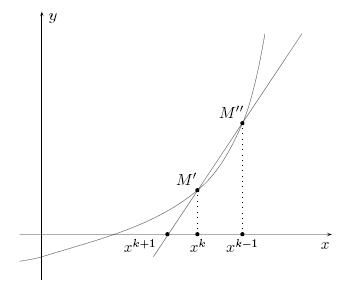
\includegraphics[scale=0.8]{img/Sekush.JPG}
$$
Такой модифицированный метод Ньютона называют меодом секущих. 
\end{document}